\documentclass[aspectratio=169]{beamer}

\mode<presentation>
\usetheme{Boadilla}
\definecolor{Columbia}{RGB}{185,217,235}
\definecolor{Columbia2}{RGB}{0,51,160}
\definecolor{Columbia3}{RGB}{0,114,206}
\definecolor{blue}{RGB}{30,90,205}
\definecolor{red}{RGB}{213,94,0}
\definecolor{green}{RGB}{0,128,0}
\setbeamercolor{title}{fg=Columbia3}
\setbeamercolor{frametitle}{fg=Columbia3}
\setbeamercolor{block title}{bg=Columbia3, fg=white}
\setbeamercolor{block body}{bg=white}
\setbeamercolor{structure}{fg=Columbia3}
\setbeamercolor{item projected}{fg=white}
\setbeamercolor{item}{fg=Columbia3}
\setbeamercolor{subitem}{fg=Columbia3}
\setbeamercolor{section in toc}{fg=Columbia3}
\setbeamercolor{description item}{fg=Columbia3}
\setbeamercolor{caption name}{fg=Columbia3}
\setbeamercolor{button}{bg=Columbia3, fg=white}
\usepackage{graphics}
\usepackage{geometry}
\usepackage{booktabs}
\usepackage{tikz}
\usepackage{amsmath}
\usepackage{bbm}
\usetikzlibrary{decorations.pathreplacing}
\usepackage{multirow, makecell}
\usepackage{float}
\usepackage{fancyvrb}
\usepackage{caption}
\usepackage{subcaption}
\usepackage{adjustbox}
\usepackage{threeparttable}
\usepackage{hyperref}
\usepackage[scaled=0.92]{helvet}
\newenvironment{wideitemize}{\itemize\addtolength{\itemsep}{10pt}}{\enditemize}
\newenvironment{wideenumerate}{\enumerate\addtolength{\itemsep}{10pt}}{\endenumerate}
\newenvironment{widedescription}{\description\addtolength{\itemsep}{10pt}}{\enddescription}
\hypersetup{
colorlinks=true,
linkcolor=blue,
filecolor=green, 
urlcolor=blue,
}
\beamertemplatenavigationsymbolsempty
\setbeamercolor{author in head/foot}{bg=white, fg=Columbia3}
\setbeamercolor{title in head/foot}{bg=white, fg=Columbia3}
\setbeamercolor{date in head/foot}{bg=white, fg=Columbia3}
\setbeamercolor{section in head/foot}{bg=white, fg=Columbia3}
\setbeamercolor{page number in head/foot}{bg=white, fg=Columbia3}
\setbeamercolor{headline}{bg=Columbia}
\setbeamertemplate{footline}{
    \leavevmode%
    \hbox{%
        \begin{beamercolorbox}[wd=.333333\paperwidth,ht=2.25ex,dp=1ex,center]{date in head/foot}%
            \usebeamerfont{date in head/foot}\insertshortdate
        \end{beamercolorbox}%
        \begin{beamercolorbox}[wd=.444444\paperwidth,ht=2.25ex,dp=1ex,center]{title in head/foot}%
            \usebeamerfont{title in head/foot}\insertshorttitle
        \end{beamercolorbox}%
        \begin{beamercolorbox}[wd=.222222\paperwidth,ht=2.25ex,dp=1ex, center]{page number in head/foot}%
            \usebeamerfont{page number in head/foot} \insertframenumber{} / \inserttotalframenumber
        \end{beamercolorbox}}%
        \vskip0pt%
    }
%\setbeamercolor{page number in head/foot}{fg=black}
\setbeamertemplate{section in toc}[sections numbered]
\setbeamertemplate{subsection in toc}{\leavevmode\leftskip=3em\rlap{\hskip-1.75em\inserttocsectionnumber.\inserttocsubsectionnumber}\inserttocsubsection\par}
\setbeamerfont{subsection in toc}{size=\footnotesize}
%\setbeamertemplate{headline}{%
  %\begin{beamercolorbox}[ht=5.5ex]{section in head/foot}
    %\vskip2pt\insertnavigation{0.33\paperwidth}\vskip2pt
  %\end{beamercolorbox}%
%}
\newenvironment{transitionframe}{\setbeamercolor{background canvas}{bg=Columbia3}\setbeamertemplate{footline}{} \begin{frame}}{\end{frame}}


\makeatletter
\let\@@magyar@captionfix\relax
\makeatother


\title[Recitation 3]{Recitation 3} % Change this regularly
\author[Seung-hun Lee]{Seung-hun Lee}
\institute[Columbia University]{Columbia University}

\date[October 11th, 2021]{October 11th, 2021}

\begin{document}
\begin{frame}
\titlepage
\end{frame}

%%%%%%%%%%%%% Section 1. 


\begin{frame}
\frametitle{Errors may have different distribution across observations}
\begin{itemize}
\item The assumption that $var(u_i)$ is constant may not hold. Thus, be open for heteroskedasticity
\item If we stick to homoskedasticity in this case, the standard errors are incorrectly estimated (usually underestimated)
\begin{figure}[H]
\centering
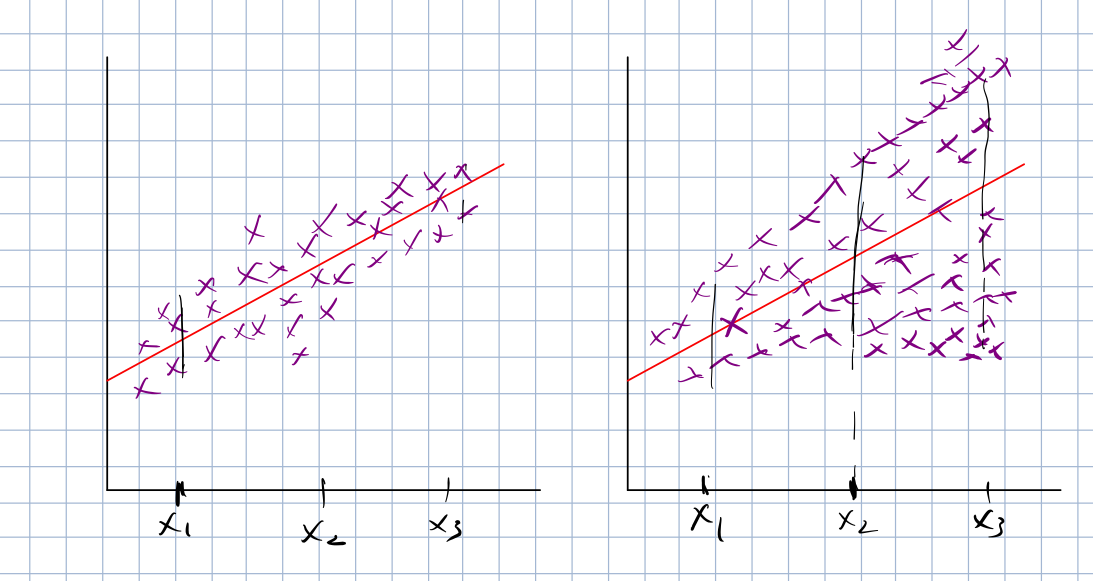
\includegraphics[width=0.55\textwidth]{hetero.png}
\end{figure}
\item  In such case, standard errors of our estimators must take this into account.
\end{itemize}
\end{frame}

\begin{frame}
\frametitle{...but what does heteroskedasticity change?}
\begin{figure}[H]
\centering
\begin{subfigure}[b]{0.49\textwidth}
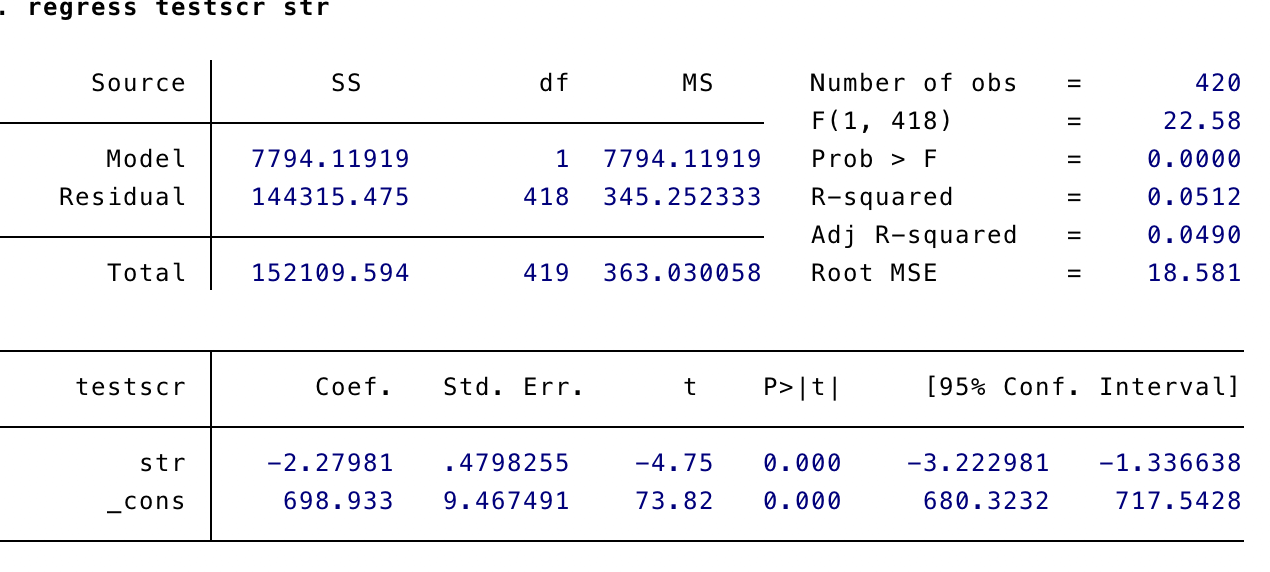
\includegraphics[width=\textwidth]{nonrobust.png}
\end{subfigure}
\begin{subfigure}[b]{0.49\textwidth}
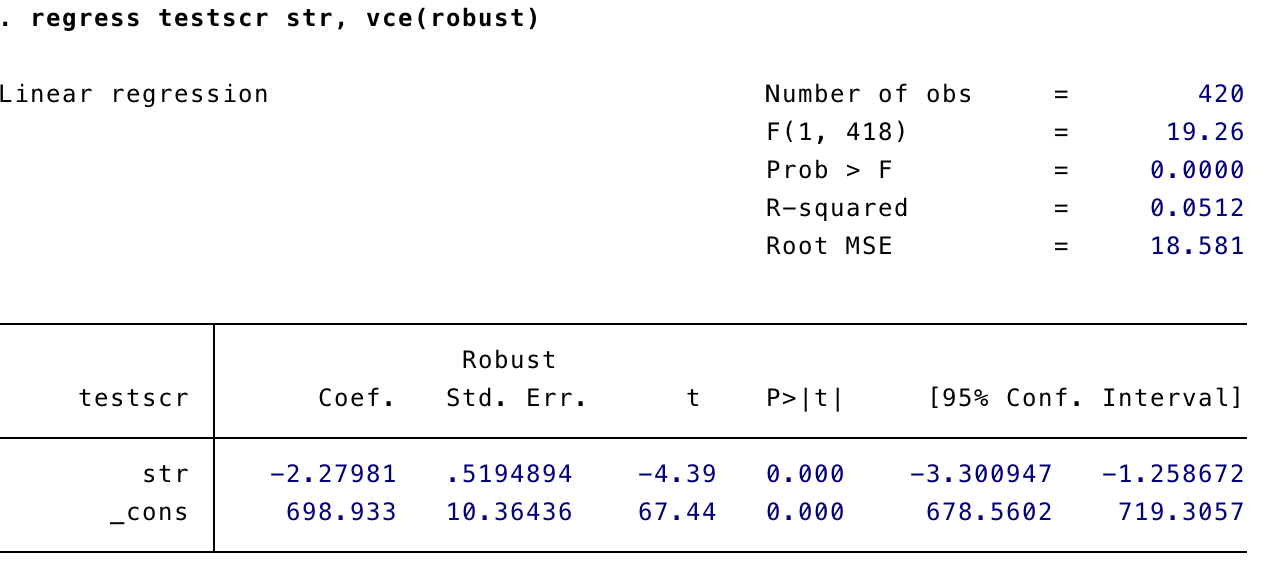
\includegraphics[width=\textwidth]{robust.png}
\end{subfigure}
\end{figure}
\begin{itemize}
\item The variance rises (usually) in the heteroskedastic regression, so we may make a wrong hypothesis test
\item The coefficients are unchanged, since estimation of OLS estimates did not rely on homoskedasticity
\end{itemize}
\end{frame}


\begin{frame}
\frametitle{Multivariate Regression: Why add more variables to the right?}
\begin{itemize}
\item Suppose that there are more than one possible independent variable
\item The set of models are
\[
\begin{aligned}
\text{True: }& Y_i = \beta_0 + \beta_1 X_i + \beta_2 Z_i+u_i\\
\text{Mistake: }& Y_i = \beta_0 + \beta_1 X_i + u_i^*\\
\text{Sample: }& Y_i = \hat{\beta}_0 + \hat{\beta}_1 X_i+ \hat{u}_i\\
\end{aligned}
\]
\item Suppose you run an OLS regression without $Z_i$.  $\hat{\beta}_1$ can be calculated as $\frac{\sum_{i=1}^n(X_i-\bar{X})(Y_i-\bar{Y})}{\sum_{i=1}^n(X_i-\bar{X})^2}$. Replacing this with the true model gives
\footnotesize{\[
\begin{aligned}
\frac{\sum_{i=1}^n(X_i-\bar{X})(Y_i-\bar{Y})}{\sum_{i=1}^n(X_i-\bar{X})^2} =& \frac{\sum_{i=1}^n(X_i-\bar{X})(\beta_1(X_i-\bar{X})+\beta_2(Z_i-\bar{Z})+(u_i-\bar{u}))}{\sum_{i=1}^n(X_i-\bar{X})^2}\\
=& \beta_1 + \beta_2\frac{\sum_{i=1}^n(X_i-\bar{X})(Z_i-\bar{Z})}{\sum_{i=1}^n(X_i-\bar{X})^2}+\frac{\sum_{i=1}^n(X_i-\bar{X})(u_i-\bar{u})}{\sum_{i=1}^n(X_i-\bar{X})^2}\\
\end{aligned}
\]}\normalsize
\end{itemize}
\end{frame}


\begin{frame}
\frametitle{Omitted variable bias: Bias from missing out needy independent variables}
\begin{itemize}
\item If $\beta_2 \neq0$ and $\frac{\sum_{i=1}^n(X_i-\bar{X})(Z_i-\bar{Z})}{\sum_{i=1}^n(X_i-\bar{X})^2}\neq 0$, then the mean of $\hat{\beta}_1$ is not guaranteed to be $\beta_1$. This leads to the \textbf{omitted variable bias} problem
\item This happens when both of the following cases hold
\begin{itemize}
\item \underline{$Z$ should explain $Y$}: If the slope coefficient of $Z$ ($\beta_2$) is nonzero, then the $Z$ variable is part of the error term if we forget to include them
\item \underline{$Z$ is correlated with $X$}: If $cov(X,Z)\neq0$ and the regression residual $\hat{u}$ is correlated with $Z$, the independent variable is now correlated with $\hat{u}$, which leads to violation of the assumption that independent variable and the residual are not correlated.
\end{itemize}
\item We can even determine the direction of the bias
\begin{itemize}
\item $\hat{\beta}_1$ is overestimated if $\beta_2\frac{\sum_{i=1}^n(X_i-\bar{X})(Z_i-\bar{Z})}{\sum_{i=1}^n(X_i-\bar{X})^2}>0$
\item $\hat{\beta}_1$ is underestiated  if $\beta_2\frac{\sum_{i=1}^n(X_i-\bar{X})(Z_i-\bar{Z})}{\sum_{i=1}^n(X_i-\bar{X})^2}<0$
\end{itemize}
\end{itemize}
\end{frame}

\begin{frame}
\frametitle{Omitted variable bias: What to do about it?}
\begin{itemize}
\item We can simply include the $Z$ variable if we have the data for it. 
\item Another way is to conduct an ideal randomized controlled experiment (or randomized control trial) that randomly assigns value of $X$ to all students.
\item If none of the two are feasible, we should find another variable that can be a proxy to $Z$ - they have to be related to the $X$ variable and is uncorrelated with the errors - which is the Instrumental Variable method.
\end{itemize}
\end{frame}

\begin{frame}
\frametitle{Multivariate regression: So now what does the coefficients really mean?}
\begin{itemize}
\item The technicalities involved do not change drastically compared to the univariate regression. 
\item However, one should interpret the coefficients cautiously. Suppose that the regression is
\[
Y_i = \beta_0 + \beta_1 X_i + \beta_2 Z_i+u_i
\]
\item To see the impact of $X_i$ and $Y_i$, one needs to take (partial) derivatives on $Y_i$ with respect to $X_i$. This leads to
\[
\beta_1 = \frac{\partial Y_i}{\partial X_i}
\]
\item In words, $\beta_1$ captures how much $Y_i$ changes with respect to $X_i$ \emph{holding other variables constant} (ceteris paribus).
\item If you do not hold other variables ($Z_i$ in this case) fixed, the change will not exactly be $\beta_1$ (it could be more or less)

\end{itemize}
\end{frame}

\begin{frame}
\frametitle{Sapling distribution of estimates: Just derive this once in your life}
\begin{itemize}
\item The estimates for the $\hat{\beta}_j$, can be obtained in a similar way in which we have obtained the OLS estimates for the single variable version.
\[
\min_{\{\beta_0,\beta_1,\beta_2\}} \sum_{i=1}^n[Y_i-\beta_0 - \beta_1X_{1i}-\beta_2X_{2i}]^2
\]
\item After some more amount of algebra (than the single variable case), the result we get is the following
\begin{itemize}
\item[$\hat{\beta}_0=$] $\bar{Y}-\hat{\beta}_1\bar{X}_1-\hat{\beta}_2\bar{X}_2$
\item[$\hat{\beta}_1=$] $\frac{\sum_{i=1}^n (X_{1i}-\bar{X}_1)(Y_{i}-\bar{Y})\sum_{i=1}^n(X_{2i}-\bar{X}_2)^2-\sum_{i=1}^n (X_{2i}-\bar{X}_2)(Y_{i}-\bar{Y})\sum_{i=1}^n(X_{1i}-\bar{X}_1)(X_{2i}-\bar{X}_2)}{\sum_{i=1}^n (X_{1i}-\bar{X}_1)^2\sum_{i=1}^n (X_{2i}-\bar{X}_2)^2-[\sum_{i=1}^n (X_{1i}-\bar{X}_1)(X_{2i}-\bar{X}_2)]^2}$
\item[$\hat{\beta}_2=$] $\frac{\sum_{i=1}^n (X_{2i}-\bar{X}_2)(Y_{i}-\bar{Y})\sum_{i=1}^n(X_{1i}-\bar{X}_1)^2-\sum_{i=1}^n (X_{1i}-\bar{X}_1)(Y_{i}-\bar{Y})\sum_{i=1}^n(X_{1i}-\bar{X}_1)(X_{2i}-\bar{X}_2)}{\sum_{i=1}^n (X_{1i}-\bar{X}_1)^2\sum_{i=1}^n (X_{2i}-\bar{X}_2)^2-[\sum_{i=1}^n (X_{1i}-\bar{X}_1)(X_{2i}-\bar{X}_2)]^2}$
\end{itemize} \par\medskip
\item What matters at this point is how we should \textbf{interpret} these coefficients. 
\end{itemize}
\end{frame}

\begin{frame}
\frametitle{What new problems do we have in multivariate regressions?}
\begin{itemize}
\item We are quite likely to end up including independent variables that are highly correlated with each other. There are two \item We say two variables $X_1$ and $X_2$ are \textbf{perfectly multicollinear} if $X_1$ is in an exact linear relationship of some sort with $X_2$.
\item Any multicollinearities that are not in exact linear relationship is referred to as \textbf{imperfect multicollinearity}. 
\end{itemize}
\end{frame}

\begin{frame}
\frametitle{When does perfect multicollinearity happen?}
\begin{itemize}
\item \textbf{Assume that $X_2 = cX_1$ for some constant $c$}: Then we have $(X_{2i}-\bar{X}_2)=c(X_{1i}-\bar{X}_1)$. Then $\hat{\beta}_1$ changes to $\frac{0}{0} $ 
\item \textbf{Dummy variable trap}: Say that you have the dummy variable for females and males. Let each of them be $X_{1i}$ and $X_{2i}$ with $X_{2i}=1-X_{1i}$. Then the regression can be written as
\begin{gather*}
Y_i = \beta_0 + \beta_1X_{1i} + \beta_2X_{2i} + u_i \iff Y_i = \beta_0 + \beta_1X_{1i} + \beta_2(1-X_{1i}) + u_i \\
\iff Y_i = \beta_0 + \beta_2 +(\beta_1-\beta_2)X_{1i}+u_i
\end{gather*}
Therefore, by including both $X_{1i}$ and $X_{2i}$ in the same regression, the $X_{2i}$ vanishes from the equation. This is why when you have dummy variables for all categories in the observation, \textbf{one of them must be left out.}
\end{itemize}
\end{frame}



\begin{frame}
\frametitle{Adjusted $R^2$ and why we need this}
\begin{itemize}
 \item Additional complication rises from interpreting the goodness of fit. In addition to $R^2$, we now get the \textbf{adjusted $R^2$} (or $\bar{R}^2$), which is defined as
\[
\bar{R}^2 = 1-\frac{n-1}{n-k-1}\frac{\text{RSS}}{\text{TSS}} \ \ (k:\text{number of independent variables})
\]
\item Since we are assuming that $k\geq 1$, adjusted $R^2$ is smaller than the $R^2$. 
\item As we include more variables, the $\frac{n-1}{n-k-1}$ increases, leading to further decrease in  $\bar{R}^2$. \\ (There is no such factor in $R^2$, so it always increases even with irrelevant variable)
\item However, if the new variables are very relevent, $\frac{\text{RSS}}{\text{TSS}}$ decreases quickly. 
\item This reduces the gap between $R^2$ and the adjusted $R^2$. If the adjusted $R^2$ do not decrease drastically, it is a sign that we are adding a relevant variable. \par\medskip
\end{itemize}
\end{frame}


\begin{frame}
\frametitle{Joint hypothesis tests (Why it is not straightforward)}
\begin{itemize}
\item Suppose that you are running a two-sided test with 5 independent variables and significance level $\alpha = 5\%$ under the null hypothesis
\[
H_0: \beta_1=...\beta_5=0
\]
\item You reject the null hypothesis when $|t_i|\geq 1.96 $ with probability 0.05. 
\item Now assume that each test statics are independent. Then the probability of incorrectly rejecting the null hypothesis using this approach is
\footnotesize{\[
\begin{aligned}
\Pr(|t_1|>1.96 \cup...\cup |t_5|>1.96) & =1-\Pr(|t_1|\leq1.96\cap .. \cap|t_1|\leq1.96)\\
(\because\text{Independence of $t_i$'s}) \ \ &=1-\Pr(|t_1|\leq1.96)\times ..\times\Pr(|t_5|\leq1.96) \\
 & = 1-(0.95)^5 \\
 &= 0.2262
\end{aligned}
\]}\normalsize
\item This means that the rejection rate under the null is not 5\% but 22\% percent - we end up rejecting the null hypothesis more than we have to.
\end{itemize}
\end{frame}


\begin{frame}
\frametitle{F-test for joint significance}
\begin{itemize}
\item This is a test where all parts of the joint hypothesis can be tested at once. It also has mechanism for correcting the correlation between the $t$-test statistics.
\item It ultimately allows us to correctly set the significance level even for the multiple testing case.
\item The usual joint hypothesis test for the regression with $k$ variables (not including the constant term) is
\[
H_0: \beta_1 = ... =\beta_k=0, \ H_1:\lnot H_0
\]
where $H_1$ refers to the case where there is a nonzero element in any one of $\beta_1$ to $\beta_k$.
\item Note that the default F-test null hypothesis for STATA is as above
\end{itemize}
\end{frame}



\begin{frame}
\frametitle{Tricks for deriving $F$-statistics}
\begin{itemize}
\item Assuming $H_0: \beta_1 = ... =\beta_q=0$ hypothesis, we use $R^2$ from the 'unrestricted' and 'restricted' regressions.
\begin{itemize}
\item Assume the following setup
\footnotesize{\[\begin{aligned}
\text{Restricted: } & Y_i =\beta_0+ 0X_{1,i} + ...+ 0X_{q,i}+ \beta_{q+1}X_{q+1,i}+...+\beta_kX_{k,i} + u_i\\
\text{Unrestricted: } & Y_i = \beta_0+\beta_1X_{1,i} + ... +\beta_qX_{q,i}+ \beta_{q+1}X_{q+1,i}+...+\beta_kX_{k,i} + u_i\\
\end{aligned}\]}\normalsize
\item Restricted regression assumes that $H_0$ is true and then only optimizes with respect to $\beta_{q+1},...,\beta_{k}$.
\item Unrestricted regression does not assume that $H_0$ is true and optimizes with respect to all slope coefficients.
\end{itemize}
\end{itemize}
\end{frame}


\begin{frame}
\frametitle{Tricks for deriving The $F$-statistic}
\begin{itemize}
 \item We use $R^2$ from these two regressions. 
\[
\frac{(R^2_{\text{Unrestricted}}-R^2_{\text{Restricted}})/q}{(1-R^2_{\text{Unrestricted}})/(n-k-1)}
\]
\begin{itemize}
\item $k$: number of independent variables (not counting intercept)
\item $q$ is the number of restrictions. 
\item Since unrestricted models allows roles for $X_1,...,X_q$ variables, they have higher $R^2$ (Restricted: They should have no role)
\end{itemize}
\item Another: Using $R^2_{\text{Restricted}} = 1-\frac{RSS_{\text{Restricted}}}{TSS}$, we can write
\[
\frac{(RSS_{\text{Restricted}}-RSS_{\text{Unrestricted}})/q}{(RSS_{\text{Unrestricted}})/(n-k-1)}
\] 
\end{itemize}
\end{frame}

\begin{frame}
\frametitle{Other tests in multivariate regressions}
\begin{itemize}
\item Suppose that instead of $\beta_1$ and $\beta_2$ being zero, we are just interested in whether they are equal.
\item The $F$-test can also be used for testing this hypothesis. The setup of the hypothesis would be
\[
H_0: \beta_1 = \beta_2 \ H_1: \beta_1 \neq \beta_2
\]
\item With this, you can answer various types of tests (e.g. is $\beta_1+\beta_2=100$?)
\end{itemize}
\end{frame}


%%%%%%%%%%%
\end{document}
